\documentclass[a4paper,12pt]{article}
\usepackage[top=2cm, bottom=2cm, left=2cm, right=2cm]{geometry}
\usepackage[nodayofweek]{datetime}
\usepackage[T1]{fontenc}
\usepackage[sc]{mathpazo}
\linespread{1.05}
\newcommand{\ver}{4.3.6}
\usepackage{setspace}
\usepackage{graphicx}
\begin{document}
\title{TARQUIN User Guide \\ Version \ver}
\author{Martin Wilson, Greg Reynolds}
\date{\today}

\maketitle

\tableofcontents

\pagebreak

\section{Preliminaries}
The latest version of this document and the TARQUIN fitting package is available from http://tarquin.sourceforge.net/. Make sure you have the latest version of the software and this guide before continuing as the package is undergoing continual improvement.  TARQUIN is currently available for the Linux and Windows platforms in two versions: the command line version most suitable to batch use and the GUI version most suitable for interactive analyses.  Finally, before using or installing TARQUIN, please read the disclaimer included at the end this document to ensure that the this package is appropriate for your purposes.

\section{Installation}
\subsection{Windows}
The Windows TARQUIN package will be supplied as a zip archive, to install the package download the file, right click on the archive and select ``Extract All...''.  This will create a new ``TARQUIN\_Windows\_\ver'' directory in the current folder.  Within this directory are the following subdirectories : ``basis\_sets'', ``example\_data'' and ``tarquin''.  To run the gui version of TARQUIN open the ``tarquin'' directory and double click on ``tarquingui.exe''.  The command line version can be run by opening the Command Prompt program and running ``tarquin.exe''.

\subsection{Mac OSX}
The OSX version of TARQUIN is bundled as a standard application. The convention is to extract the dmg file and copy the tarquingui bundle to the Applications folder. The bundle also contains the command-line version of tarquin. To use the command line version run the following:

{\tt export PATH=\$PATH:/Applications/tarquingui.app/Contents/MacOS}

This will add the tarquin binaries to the path assuming the tarquingui bundle has been copied the standard Applications folder. This line can also be added to the local .bashrc file to avoid the need to type it every time a new terminal is opened.

\subsection{Linux}
The Linux TARQUIN package will be supplied as a tar.gz archive.  Download the file and open up a terminal.  Navigate to the directory containing the archive and uncompress using the following commands : \\
{\tt cd my\_download\_directory \\
tar -zxvf TARQUIN\_Linux\_\ver.tar.gz} \\
To run the TARQUIN gui enter the ``tarquin'' directory and execute ``tarquingui'' : \\
{\tt cd TARQUIN\_Linux\_\ver/tarquin \\
./tarquingui } \\
the command line version can also be run as follows : \\
{\tt ./tarquin}

\section{GUI User Guide}
\subsection{Quick analysis}
Upon starting the TARQUIN GUI, you will be greeted with a blank plotting window and a menubar located at the top of the window. To perform a basic analysis select ``File'' then ``Quick fit...'' or alternatively press ``q''.  At this point you can select your water suppressed data file and water reference data file where appropriate.  For a first attempt, try to fit the example data included in the ``example\_data'' directory. In this case choose the ``philips\_spar\_sdat\_WS.SDAT'' file as the water suppressed scan and the ``philips\_spar\_sdat\_W.SDAT'' file as the water unsuppressed scan.

TARQUIN will automatically try and guess the format of the data but if this fails then you may be prompted to select the data format manually.  Once the input data is correctly specified select the Fit button.  At this stage TARQUIN will perform the following steps:
\begin{enumerate}
\item Simulate a PRESS basis set based on the parameters in the data file. 
\item Remove the residual water signal.
\item Perform a preliminary phase estimation.
\item Calibrate the PPM axis based on spectral features.
\item Fit the data.
\end{enumerate}

Steps 2-4 are known as preprocessing.

\subsection{Viewing and saving fit results}
Once the fitting process is completed the concentrations of the measured signals will be displayed, to view the fit plot select ``ok''.  The window should look like Figure \ref{eg_plot} with a plot of the fitted signals and a legend to the right.  Signals can be added and removed from the plot by selecting their names in the legend and selecting two points on the plot with a single left mouse click of the mouse will create a zoom region.  A single right mouse click will return the axes limits to their previous values. Pressing ``x'' or ``y'' will show the full scale in the x and y directions of the plot.

\begin{figure}[h!]
\centering
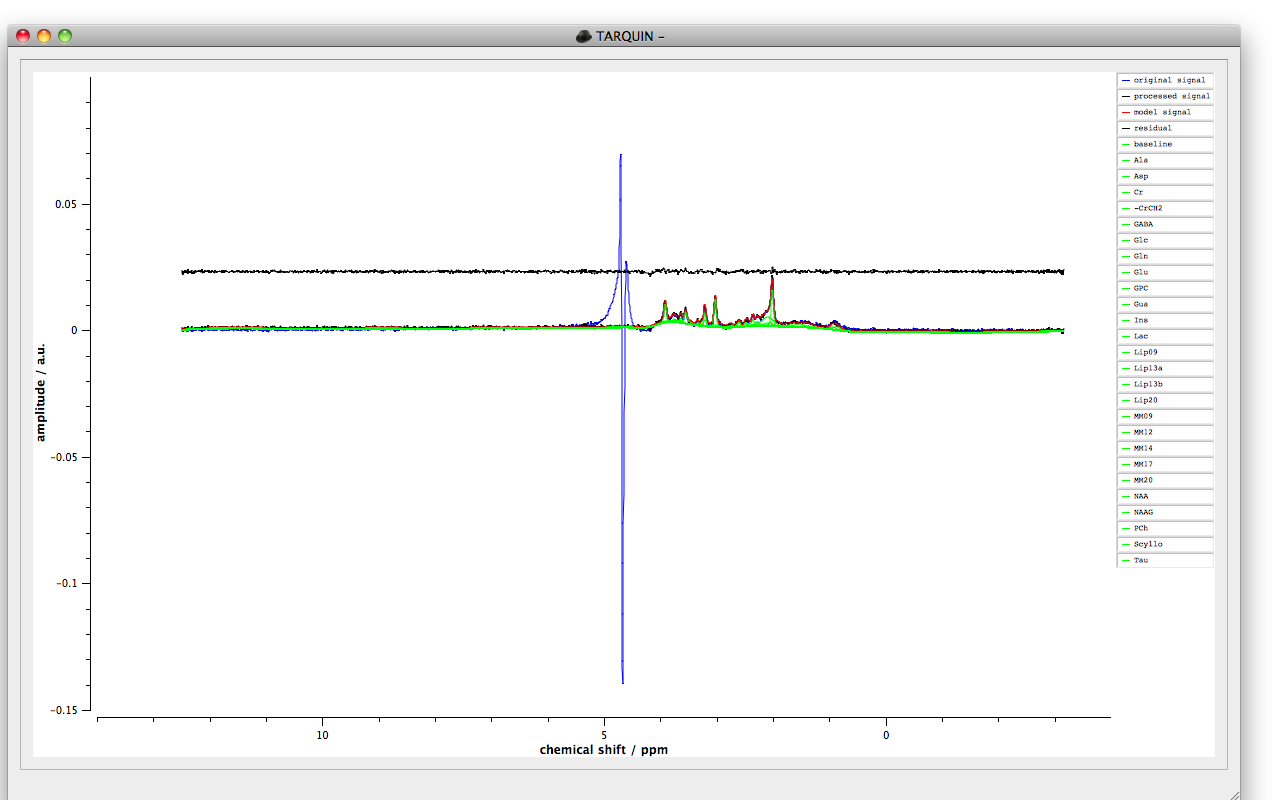
\includegraphics[width=\textwidth]{figs/fit_example.png}
\caption{An example fit plot.}
\label{eg_plot}
\end{figure}

Once the fit has been performed it can be useful to save the results and/or export the signal amplitudes for further analysis. To export the fit as a pdf file select the ``Export plot...''.  The signal amplitudes can also be exported in a formatted text or csv format using the ``Export TXT...'' and ``Export CSV results...'' options respectively from the ``Results'' menu.  Alternatively a table of signal amplitudes can be displayed using by selecting the ``Fitted amplitudes'' option or by pressing the ``r'' key.

\subsection{Advanced analysis}
The quick fit procedure is useful for routine analysis of PRESS data but unsuitable in cases where the default options need to be adjusted.  In these cases the advanced fit dialogue should be opened by selecting ``File'' followed by ``Advanced fit...'' or by pressing the ``a'' key.  A screen shot of the advanced fit dialogue is given in Figure \ref{adv_fit}.

\begin{figure}[h!]
\centering
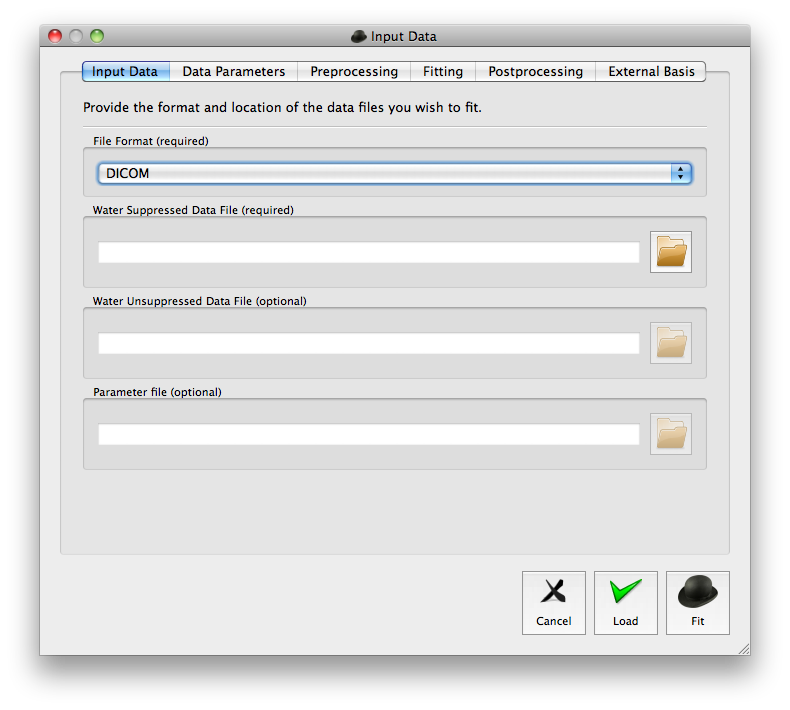
\includegraphics[width=\textwidth]{figs/adv_fit.png}
\caption{The advanced fit window.}
\label{adv_fit}
\end{figure}

Unlike the quick fit procedure the data format must be selected prior to selecting the input data files.  Once the data has been successfully read the basic acquisition parameters are displayed in the ``Data Parameters'' tab.  These can be manually edited in case of incorrect parameter detection.  The pulse sequence is assumed to be PRESS but can be easily changed via the ``Pulse sequence'' combination box. Once the correct options have been set, the user can load the data to view without any processing using the ``Load'' button. Alternatively, choosing the ``Fit'' button will perform the analysis and display the results.

If the data was loaded with the ``Load'' button the user can choose to pre-process the data and perform a full analysis using the ``Analysis'' menu in the main window.

\section{Command Line User Guide}
\subsection{Unix-like}
All Unix-like operating systems have access to a terminal application which allows commands to be entered. Finding and running the terminal application is specific to the flavour of Unix you are using, but should be simple enough.  If you are new to the Unix command line and would like some help, http://linuxcommand.org is a decent place to start.

Once you have installed TARQUIN it is recommended (for convenience) that the location of the tarquin binary is on your path.  This means that typing \texttt{tarquin} on the command line should start the program irrespective of the current working directory.  To do this on a temporary basis type the following at the command line:
\\
\\
\texttt{export PATH=\$PATH:your\_path\_to\_binary}
\\
\\
To add the path automatically each time a terminal is opened, add the line to the .bashrc file located in your home directory.

%\subsection{Windows}

\subsection{Example Usage}
The command line version of TARQUIN requires the used to specify options to the software using a series of arguments to the main program.  The options are specified in the following way:
\\
\\
\noindent
\texttt{tarquin ---option1 value1 ---option2 value2 ---option3 value3...}
\\
\\
An example command follows which will fit the \texttt{WS.ima} data file using \texttt{W.ima} as a water reference file.  The data format is specified to be Siemens ima and a text file of results is outputted.
\\
\\
\noindent
\texttt{tarquin ---input WS.ima ---input\_w W.ima ---format siemens}

\noindent
\texttt{---output\_txt results.txt}
\subsection{Common TARQUIN Parameters}

\begin{tabular}{l l}
Option & Description \\
\hline
\texttt{input} & Water suppressed input file (required). \\
\texttt{input\_w} & Water unsuppressed reference file (required for ``absolute'' quantitation). \\
\texttt{output\_csv} & Output a csv file of the determined signal quantities. \\
\texttt{output\_txt} & Output a text file of the determined signal quantities. \\
\texttt{format} & Data format (this can usually be determined automatically for the main \\ 
& clinical data formats). \\
\texttt{basis\_csv} & The directory containing a csv representation of the basis set.\\
%& unless \texttt{basis\_xml} has been specified). \\
\texttt{output\_pdf} & Output a pdf plot of the fit results, this option requires gnuplot. \\
\texttt{ext\_pdf} & \{true, false\} Extended pdf plot of the fit results showing individual basis signals. \\
\texttt{output\_fit} & Output a text file of the fit results, useful for producing fit plots in \\ 
& external software. \\
\texttt{output\_basis} & Output a precomputed basis set file, this file should only be applied to \\ 
& data with identical experimental parameters to the data from which it \\
& was generated. \\
\texttt{w\_conc} & Unsuppressed water concentration in mM, see $water_{conc}$ in section \ref{ws}.\\ 
\texttt{w\_att} & Water scaling attenuation factor, see $water_{att}$ in section \ref{ws}.\\ 
\end{tabular}
\\
\\
\\
\noindent
\begin{tabular}{l l}
Format & Description \\
\hline
\texttt{siemens} & Siemens IMA. \\
\texttt{rda} & Siemens RDA. \\
\texttt{philips} & Philipis SPAR/SDAT. \\
\texttt{ge} & GE P-file. \\
\texttt{shf} & GE shf file accompanying a P-file. \\
\texttt{dcm} & DICOM spectroscopy. \\
\texttt{varian} & Varian fid format. \\
\texttt{bruker} & Bruker fid format. \\
\texttt{jmrui\_txt} & JMRUI ASCII format. \\
\texttt{dpt} & Dangerplot ASCII format. \\
\end{tabular}

%\subsection{The Parameter File}
%Nothing yet.

\subsection{Automated Analysis}
Since TARQUIN analyses can be performed from the command line, the batch analysis of spectra can be performed with the aid of a scripting language.  If you are using a Unix-like OS and have some experience with the command line then bash is a good scripting language to start with.  However bash can be a little awkward to use in Windows, so an example using Python will be given as it is cross-platform and clear to read.  Instructions on how to install and use Python can be found from www.python.org.

The following code listing gives an example of how a script to automatically analyse MRS data may look:
\begin{verbatim}
#!/bin/python

import os
import sys
import re

format = 'siemens'
dir = '/home/tarquin/Desktop'
pattern = '.*MRS$'

# find all files in the dir
fileList = []
for root, subFolders, files in os.walk(dir):
    for file in files:
       fileList.append(os.path.join(root,file))

# find files that match the regex pattarn
fileListMatch = []
for file in fileList:
    if re.search(pattern,file):
        fileListMatch.append(file)

# for each matched file
for file in fileListMatch:
    command = ('tarquin --input ' + file + ' --format ' + format + 
        --output_pdf ' + file + '.pdf' + ' --output_txt ' + file + '.txt')
    # run the command
    os.system(command)
\end{verbatim}
This script recursively searches for all files within in the \texttt{dir} variable.  Each file that ends with the letters \texttt{MRS} is considered to be a data file and is stored in the \texttt{fileListMatch} vector.  TARQUIN is then run on each data file, using the default brain basis set, assuming the data is in the Siemens format.  TARQUIN outputs a pdf plot of the fit and a text file containing the metabolite quantities with the same name at the data file appended with the extensions .pdf and .txt respectively.  Where the analysis of large datasets is required, scripting can be a very useful tool for saving you a huge amount of time and wrist strain!

\section{Output parameters}
Below is a table to define some useful parameters available from the TARQUIN results output.
\vspace{\baselineskip}

\begin{tabular}{l l}
Parameter & Description \\
\hline
\texttt{Q} & standard deviation of the fit residual (between around 0.5-4 PPM) \\& divided by the standard deviation of the noise region. \\
\texttt{SNR} & ratio between the maximum in the spectrum minus baseline \\& divided by 2xRMS of the residual between 0.5-4 PPM. \\
\texttt{SNR max} & ratio between the maximum in the spectrum minus baseline \\& divided by 2xRMS of the spectral noise level. \\
\texttt{SNR metab} & ratio between the maximum in the spectrum minus baseline \\& divided by 2xRMS of the residual in the metabolite region \\& (1.9-4.0ppm) to exclude lipids from biasing the value. \\
\texttt{spec noise} & estimate of the spectral RMS noise level. \\
\texttt{init beta} & initial estimate of T2* prior to fitting. \\
\texttt{final beta} & final estimate of T2* determined during fitting. \\
\texttt{final beta (PPM)} & as above in units of PPM.\\
\texttt{water width (Hz)} & FWHM width of water peak in units of Hz where available. \\
\texttt{water width (PPM)} & As above in units of PPM. \\
\texttt{water freq (Hz)} & Difference between water frequency and the centre of the spectral \\& width in Hz. \\
\end{tabular}

\section{PDF output and quality control}
A PDF plot of the fit and fitting parameters can be exported in the GUI and command line versions of TARQUIN. Gnuplot is required for this type of output and should be on the system path (otherwise \texttt{gnuplot} option should be set). The following options relate to the PDF output:

\vspace{\baselineskip}
\begin{tabular}{l l}
Parameter & Description \\
\hline
\texttt{output\_pdf} & file name of PDF output. \\
\texttt{gnuplot} & set the path of Gnuplot (required if Gnuplot is not on the system path). \\
\texttt{ext\_pdf} & (true/false) produce a page of output for each metabolite. \\
\texttt{lb} & line broadening in Hz (cosmetic change only). \\
\texttt{ppm\_left} & change the left side of the plot axis limit. \\
\texttt{ppm\_right} & change the right side of the plot axis limit. \\
\texttt{title} & add a title to the plot (enclose between quotes). \\
\texttt{gnuplot\_cex} & text size scaling parameter. \\
\end{tabular}

\vspace{\baselineskip}
At the bottom right of the PDF output there is a section named \texttt{QC INFORMATION}. This section can act as a useful data quality guide for most MRS data. However, precise QC requirements are problem specific, so this should only be used as a guide. The criteria are set as follows:

\vspace{\baselineskip}
\begin{tabular}{l l}
Lineshape criteria & QC \\
\hline
metabolite FWHM > 0.1PPM & fail \\
0.1PPM > metabolite FWHM > 0.75PPM & pass (borderline) \\
0.075PPM > metabolite FWHM > 0.05PPM & pass (average) \\
0.05PPM > metabolite FWHM & pass (good) \\
\end{tabular}

\vspace{\baselineskip}
\begin{tabular}{l l}
SNR criteria & QC \\
\hline
4 > SNR & fail \\
10 > SNR > 4 & pass (borderline) \\
20 > SNR > 10 & pass (average) \\
SNR > 20 & pass (good) \\
\end{tabular}

\section{Data types}
\subsection{PRESS}
\subsubsection{Timings and simulation}
The standard PRESS sequence consists of two spin echoes, known as TE1 and TE2, and the summation of these times is equal to the total echo-time TE. To get the most accurate results, the simulation routine needs to know the correct TE1 and TE for your data, TE2 is determined from TE-TE1. The default TE1 can vary between manufacturers and also for different pulse shapes so it is worth finding out what pulse timings your system is using.

\subsubsection{Chemical shift displacement}
Chemical shift displacement (CSD) is an issue for all localisation methods that use the combination of an RF pulse and gradient to perform selective excitation. Generally the effects are small, however for PRESS at high field (3T or greater) CSD can become a problem \cite{CSD}. The current TARQUIN simulation routine does not take into account the influence of CSD on metabolite signals \cite{high_f_sims}, therefore if CSD is significant your results may be biased.

\subsection{High-field/rodent}
You will most likely need to reduce the ``Start point'' parameter in the ``Fitting'' tab in the advanced fit dialogue.  The equivalent command line parameter is ``start\_pnt''. TARQUIN tries to guess a decent value but if your shim or SNR is poor the fit may benefit from a lower value.

\subsection{Phantom measurements for QC analysis}
A number of centres choose to run regular phantom experiments to help identify changes in data quality that require closer investigation from the MR vendor. TARQUIN analysis of MRS performed on phantoms can provide quantitative user independent results well suited to tracking the performance of MR systems over time. The following options should be changed to ensure correct analysis of phantom data:

\begin{enumerate}
\item The starting PPM reference value should be changed from 4.65 to 4.85, due to the strong chemical shift dependence of water on temperature.
\item The PPM reference signal should be changed to NAA (assuming the phantom has appreciable levels).
\item The starting point for analysis can be reduced (10 data points should be fine), since phantom data should not have significant baseline distortion.
\item The basis set should be changed to match the chemicals in the phantom. Due to the popularity of the GE ``braino'' phantom, a predefined internal basis set can be specified as an option.
\item If the water reference method of absolute quantitation is required the \texttt{w\_conc} and \texttt{w\_att} values should be changed according to section \ref{ws}.
\end{enumerate}

Below is a series of options should be specified for a basic analysis:

\noindent\hrulefill
\begin{verbatim}
ref 4.85
start_pnt 10
ref_signals 1h_naa
int_basis braino
w_conc 55556
w_att 0.7
\end{verbatim}
\noindent\hrulefill

Please note that the ``braino'' internal basis set assumes chemical-shift and J-coupling values that may be slightly incorrect for room temperature phantoms. However any bias will be consistent between repeats and reasonable results can be obtained.

For assessing data quality, the following parameters (given in the csv results output) are worth noting for significant changes:
\begin{enumerate}
\item Water width - assesses homogeneity of the magnetic field.
\item Q - assesses the ratio between the fit residual and the noise level. A significant increase may be indicative of an artefact, a significant decrease could be related to a drop in SNR or magnetic field homogeneity.
\item SNR max - assess the ratio between the maximum metabolite signal height and the noise level. Reduction in SNR could be related to poorer homogeneity of the magnetic field or failure of a particular coil element.
\end{enumerate}

\begin{figure}[h!]
\centering
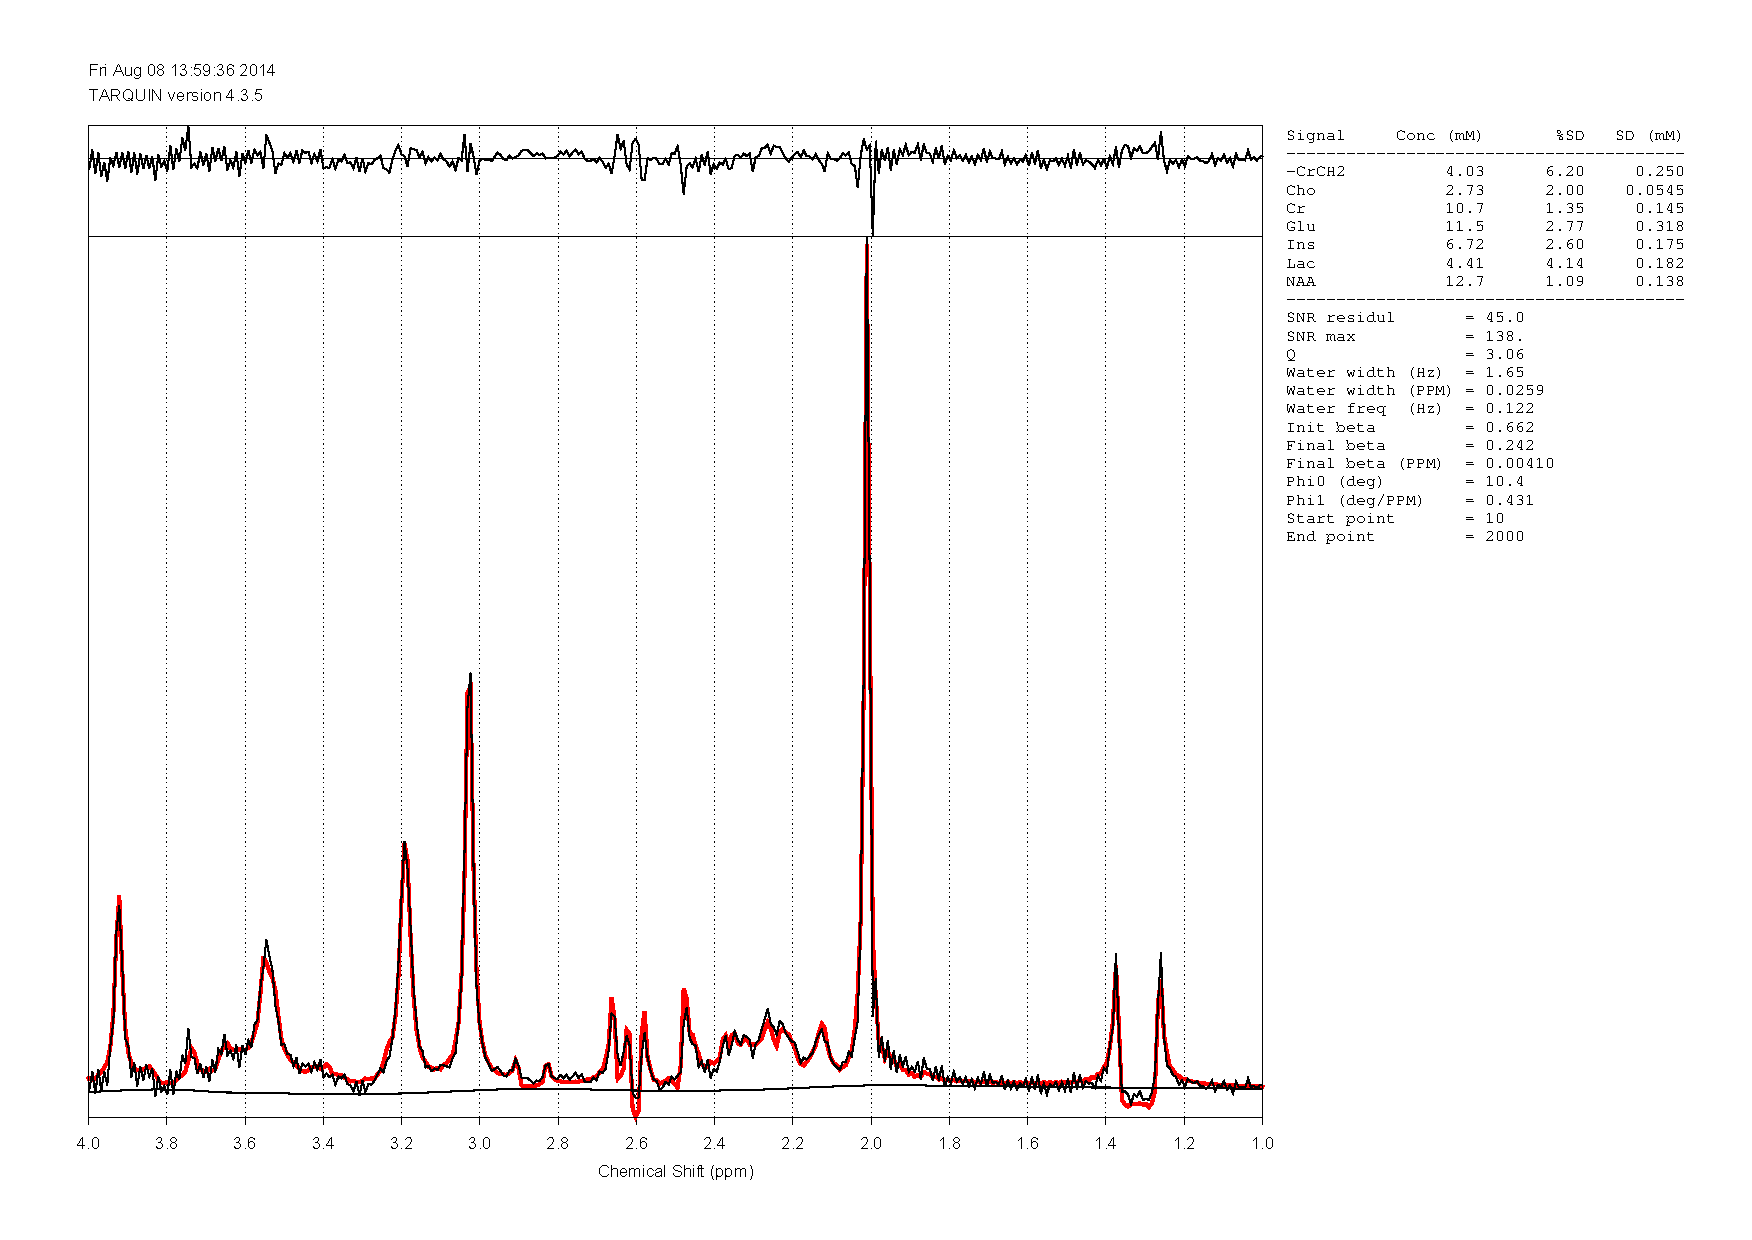
\includegraphics[width=\textwidth]{figs/braino_fit.pdf}
\caption{An example fit to the braino phantom (1.5T, PRESS TE=30ms).}
\label{braino_fit}
\end{figure}


\subsection{MEGA-PRESS}
A basic MEGA-PRESS analysis to estimate the concentration of GABA can be performed using TARQUIN. To perform analysis using the gui take the following steps:

\begin{enumerate}
\item Open the advanced fit dialogue and specify the input data in the usual way.
\item In the ``Data Parameters'' tab set the pulse sequence to ``MEGA-PRESS''. Note, this isn't a true MEGA-PRESS simulation but rather tells TARQUIN that the auto-phasing algorithm needs to expect a large negative peak.
\item To correct for frequency drift tick `Dynamic freq. correction'' and set ``Dynamic corr. ref. signals'' to ``1H Cr Cho'' or ``1H H2O'' depending on whether you have a stable residual water peak. If you choose to try this optional step always compare your results to those without the correction, this step should improve SNR/lineshape but if the scans are noisy it may degrade quality. Note, this is only worth trying if you data has been collected dynamically.
\item In the ``Preprocessing'' tab set ``Reference signals'' to ``1H NAA''. Because NAA is a prominent singlet it can be used to help the optimiser find a good value for the linewidth.
\item In the ``Fitting'' tab change the ``Start point'' to be around 10 if your sampling frequency is around 2000.
\item In the ``Fitting'' tab set ``Internal basis set'' to ``1H MEGA-PRESS GABA'' to generate a basic model of the important peaks.
\end{enumerate}

GABA is modelled as two separate peaks GABA\_A and GABA\_B, the amplitudes of these should be summed to give an estimate of the overall amount of GABA.  Note, water scaling is still performed as described in section \ref{ws} which is unlikely to be correct for MEGA-PRESS. No attempt is made to separate GABA from macromolecules at 3ppm.

Depending on how the sequence was implemented, the ``Dynamic averaging'' scheme in the ``Data Parameters'' tab may need to be set to ``Subtract even from odd'' to get a correctly combined MEGA-PRESS spectrum.

Edit on and off scans can be visualised/analysed separately by changing the ``Dynamic averaging'' scheme which can be useful for getting ratios to creatine or measuring glutamate. Furthermore, individual dynamic scans can be processed by setting the averaging scheme to ``No averaging''. Flicking through the individual scans with an eye on peak positions can be useful for detecting motion or field drift.

In some cases it may be required to separate out individual dynamics for analysis. A text file containing a list (one per line) of dynamic scans to include in the analysis can be specified with the \texttt{---av\_list} option. A file to average the first, third, fifth and seventh pairs of dynamic scans may look like the following:
\begin{verbatim}
1
2
5
6
9
10
13
14
\end{verbatim}

Typical options for MEGA-PRESS analysis are listed as follows:

\noindent\hrulefill
\begin{verbatim}
start_pnt 10
ref_signals 1h_naa
int_basis megapress_gaba
pul_seq mega_press
dyn_freq_corr true          # optional but may improve SNR
dref_signals 1h_cr_cho      # as above
dyn_av all                  # may need to be 'subtract', use 'odd' or 'even'
                            # to select edit-on/edit-off scans
av_list av_file.csv         # optional - used for selecting dynamics prior
                            # to averaging
\end{verbatim}
\noindent\hrulefill

\section{Data formats}
\subsection{GE p-files}
TARQUIN will read GE SVS p-files and combine data from multi-coil arrays where appropriate. A single phase and multiplicative factor (per coil) is applied to data from each coil before combination. Where water unsuppressed data is available this factor is taken from the phase and magnitude of the first data point in the first unsuppressed frame. Where only water suppressed data is available, this phase factor is taken from the first data point in the first suppressed frame.

\section{MRSI}
TARQUIN supports most 2D and some 3D MRSI data formats and may be used to generate metabolite maps for display on conventional MRI. Due to the relatively low resolution of MRSI, it is often useful to spatially interpolate data to allow examination of spectral data centred on pathology. This can be achieved in the gui by specifying a ``Zero fill k-space factor'' in the preprocessing tab or with the \texttt{---zfill\_kspace} command line option. In both cases the factor will be used to multiply the native resolution, so a 16x16 grid with a zero fill k-space factor of 4 will result in a 64x64 grid. Please note that this step does not improve the resolution of the technique but provides a natural method for data interpolation that will preserve the underlying point-spread function.

Following interpolation, a single voxel from the grid may be selected for analysis (``Select none'' button followed by right mouse click on the relevant voxel) and a pdf fit output can be generated from the results menu. Alternatively a set of voxels may be selected to generate metabolite maps over a region.

%\section{Fitting Details}
%The main algorithmic details and validation is described in the following paper: \cite{tarquin_paper}.  Any expansions and changes to the original algorithm will be described in the following section.

\section{Basis sets}

\subsection{Exporting LCModel .basis files}
The gui and command line (option \texttt{---output\_basis\_lcm}) versions may be used to export basis sets into a format that may be used with LCModel. By default, LCModel uses the CH3 signal from creatine to automatically scale the basis set. This frequency-domain calculation may be sensitive to signal truncation issues. Therefore when a simulated basis set is exported, the simulation is performed twice, once for the TARQUIN analysis and once for the .basis export. To avoid signal truncation errors in the LCModel basis scaling, a larger number of points to export may be specified using the \texttt{---lcm\_basis\_pts} parameter (4096 by default).

TARQUIN will not export the lipid, macromolecule or inverted CH2 creatine signals.

\subsection{Importing LCModel .basis files}
The gui and command line (option \texttt{---basis\_lcm}) versions may be used to import basis sets generated by TARQUIN or other MRS alysis packages. The basis file field strength, echo time, sampling frequency (dwell time) must all match the MRS data undergoing analysis. Where the number of points differ between the basis set and MRS data, TARQUIN will truncate or zero-fill as appropriate.

It is assumed that all metabolites in the basis file are scaled consistently and at the correct frequency (ISHIFT is ignored). It is also assumed that the signals are completely ``clean'' with no residual water or reference signals present. The centre frequency is assumed to be 4.65PPM. Finally, the basis set is not automatically scaled so this adjustment needs to be applied manually (contact me if you want to do this but don't know how or why). Whilst in principle it is possible to use experimental basis sets with TARQUIN using the .basis format, data will need to be filtered, scaled and shifted first. Simulated basis sets will be much simpler to import as these corrections are generally not required.

TARQUIN will append the lipid, macromolecule or inverted CH2 creatine signals to an imported .basis file.

\section{Absolute quantitation and water scaling}
\label{ws}
If an unsuppressed water signal is specified in TARQUIN the resulting metabolite amplitudes will be scaled to be in units of mM.  The following section describes how this is performed and what assumptions are made.
The following equation describes the relationship between the concentration of a molecule and its MRS signal:
\begin{equation}
signal_{conc} = \frac{C * signal_{amp}}{signal_{protons}}
\end{equation}
where $signal_{conc}$, $signal_{amp}$ and $signal_{protons}$ represent the concentration, amplitude and number of contributing protons of a particular signal. The constant $C$ is an unknown scaling factor. Since $signal_{protons}$ is accounted for by the simulation routine it can be disregarded from the following analysis.

The same relationship is true of water, however an attenuation factor $water_{att}$ may be required to account for the reduction of the water signal relative to the metabolites signals due to differences in T2 relaxation.
\begin{equation}
water_{conc} = \frac{C * water_{amp}}{water_{protons} * water_{att}}
\end{equation}

Since we know the water signal originates from two protons, $water_{protons}$ will be set to two.  Taking the previous two equations and substituting $C$ allows $signal_{conc}$ to be expressed as follows:

\begin{equation}
signal_{conc} = \frac{signal_{amp} * water_{conc} * water_{att} * 2}{water_{amp}}
\end{equation}

$signal_{amp}$ and $water_{conc}$ are calculated from the data. $water_{att}$ is assumed to be a constant and can be estimated from the $T_2$'s of water and metabolites as follows:

\begin{equation}
water_{att} = \frac{\exp(-t/T_2^{water})}{\exp(-t/T_2^{signal})}
\end{equation}

At 1.5T the T2 of water is approximately 80ms, and metabolites are around 400ms (although considerable variation exists between metabolite resonances). Further T2 estimates can be found in the following references \cite{metab_t2_3t,water_relaxation}. For an echo time of 30ms the correction factor can be calculated as follows:
\begin{equation}
water_{att} = \frac{\exp(-30/80)}{\exp(-30/400)} \approx 0.7
\end{equation}
Therefore the default value of $water_{att}$ is therefore 0.7 and should be modified for longer/shorter echo times or different field strengths. $water_{conc}$ represents the NMR visible water concentration (mM) and has a default value of 35880 which assumes a white matter value. 43300 and 55556 should be used for grey matter and phantoms respectively. A more in-depth discussion of the assumptions made is described in papers by Ernst et al \cite{water_ref} and Gasparovic et al \cite{csi_water_ref}.


\section{Troubleshooting}
\subsection{The baseline is unrealistic and the fit looks poor}
Try reducing the ``Start point'' parameter in the ``Fitting'' tab in the advanced fit dialogue.  The equivalent command line parameter is ``start\_pnt''. TARQUIN tries to guess a decent value but if your shim or SNR is poor the fit may benefit from a lower value.

\subsection{The basis set looks wrong}
Double check the echo time and ensure you are entering the correct value in seconds (not milliseconds) when the data is loaded.

\subsection{The ppm scale looks incorrect}
This can happen in phantom studies where the assumption that the water peak is around 4.7ppm fails. Try adjusting the ref parameter in the advanced fit dialogue.

%\subsection{Fit Quality}

%\subsection{Bugs and Features}

\section{FAQ}
Q. Is TARQUIN CE marked?\\ 
A. No. \\
Q. Will the software remain free? \\
A. Yes. \\
Q. How should I cite TARQUIN in my paper? \\
A. Please use the following reference \cite{tarquin_paper}. \\
Q. What data format is the best for using with TARQUIN? \\
A. DICOM MRS.

\section{Disclaimer}
TARQUIN is provided strictly as a research (not a clinical) tool.  The TARQUIN Package is provided ``as is'' without warranty of any kind, either expressed or implied, including (but not limited to) the implied warranties of merchantability and fitness for a particular purpose. The entire risk as to the quality and performance of the Package is with you. Should the Package prove defective, you assume the entire cost of all necessary repair or correction.

In no event will the software authors be liable to you for any damages, including lost profits, lost savings, or other incidental or consequential damages arising from the use of or the inability to use the Package (whether or not due to any defects therein) even if the authors have been advised of the possibility of such damages, or for any claim by any other party. 

\bibliographystyle{ieeetr}
\bibliography{main}

\end{document}
